\section{REST Interface}
This REST APIs were generated using \textit{Swagger Editor} and the functionalities implemented are:

\begin{itemize}
	\item \textbf{GET}:
		\subitem \textit{containers/} : Retrieve the list of all containers with their informations. The \textit{response} is a list of containers containing for each one its hostname, its name, its status and if it is monitored or not.
	\item \textbf{POST}:
		\subitem \textit{containers/\{hostname\}/\{containerName\}} : Monitor container specified in the path
	\item \textbf{DELETE}:
		\subitem \textit{containers/\{hostname\}/\{containerName\}} : Unmonitor container specified in the path
	\item \textbf{PUT}:
		\subitem \textit{/threshold} : Update the packet loss threshold used in the Agent. The value is specified in the body of the request and its type is \textit{double}.
\end{itemize}

\noindent The REST Interface makes use also of a model for specifying the structure of a Container, which is the following\footnote{the asterisk indicates that the attribute must be set}:

\begin{figure}[H]
	\begin{subfigure}{\textwidth}
	\centering
		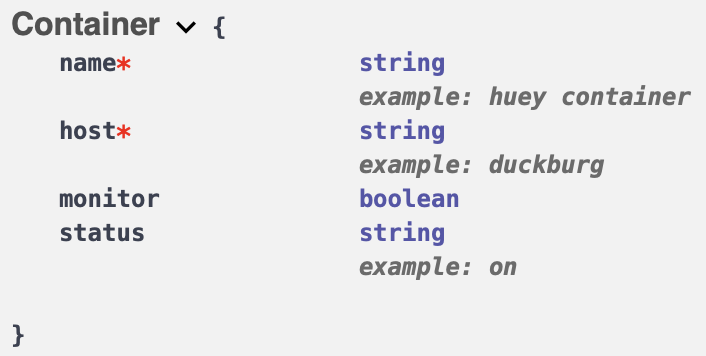
\includegraphics[width=0.9\linewidth]{img/container.png} 
	\end{subfigure}
\end{figure}